\chapter{手机传感信号和点击识别}
\label{cha:sensing} %47和30 940frame
本章将对使用的手机传感信号以及点击识别算法流程做出详细的介绍。在第~\ref{cha:intro}~章中,我们提到本工作主要是基于iPhone 11,因此本章中描述的参数主要适用于iPhone 11,如果将同样的算法移植到其他平台上可能需要对其做一定的调整。

\section{声音信号的处理}
我们获取的声音信号是线性PCM编码格式,采样率为44100Hz。软件得到的是47Hz,每次940帧的数据流,我们需要从此数据流中识别出用户触发的点击。一次点击的声音特征一般比较明显,通常是持续时间较短。另外,除去响度较大的杂音,点击峰值明显高于环境中的其他噪音。图~\ref{fig:sound-comp}给出了点击某次用户点击前后声音波形图的对比。

\begin{figure}[h]
  \centering%
  \subcaptionbox{无点击的声音波形} %标题的长度,超过则会换行,如下一个小图。
    {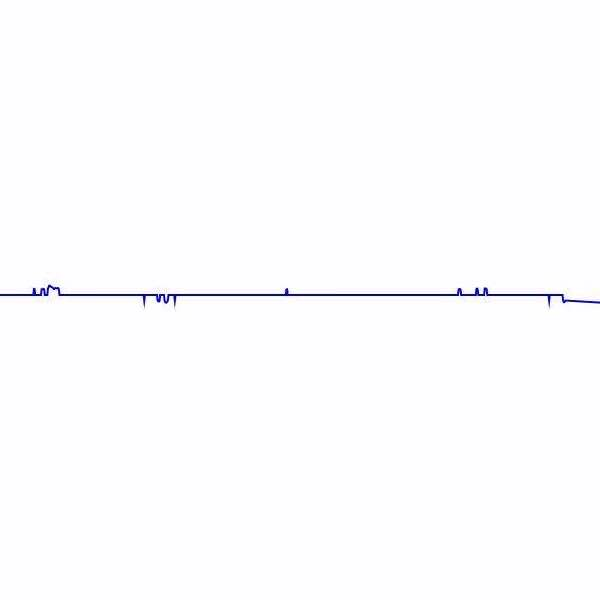
\includegraphics[height=4cm]{sound1.jpeg}}%
  \hspace{4em}%
  \subcaptionbox{某次点击的声音波形}
      {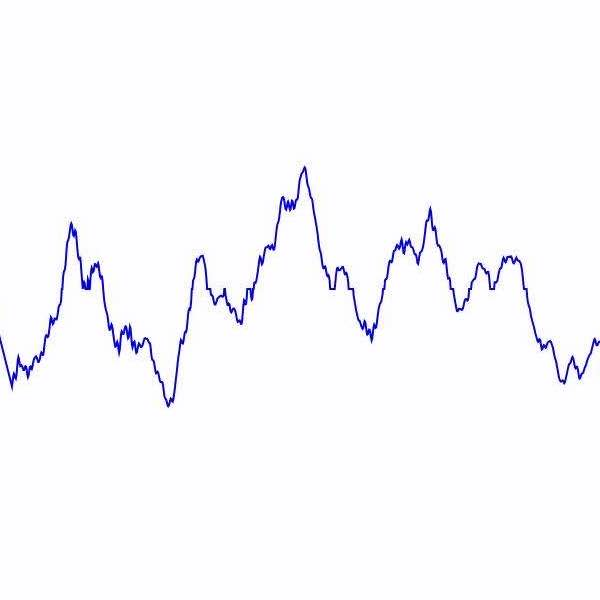
\includegraphics[height=4cm]{sound0.jpeg}}
  \caption{有无点击的声音波形对比}
  \label{fig:sound-comp}
\end{figure}

可以看出,正常无点击时波形较平,环境噪音只有很小的干扰。但是发生点击时,波峰波谷十分明显。因此,可以通过计算在一段时间窗口内数据流中超过某个阈值的数据个数判断是否有点击发生。

每帧的数据为两个字节,根据我们的经验,周围声音的响度一般低于1000,正常点击的峰值会大于3000,最终我们将3000设为阈值。此外,为了减少误识别,我们还将两次点击的最小间隔设置成50ms。通过预实验,发现除了环境中有十分类似点击的其他声音外,正常情况下该阈值的设定能够准确地识别用户的点击。

\section{深度数据的处理}
深度数据是支持我们此项工作的核心,手机前置深度数据使得任意桌面上文本输入的从全新的角度大大增加了可能性。

我们获取的数据为30Hz,维度为640*480的深度图像,其中每个像素点的数值代表手机离该点的距离。图~\ref{fig:depth1}中展示了用户端坐在手机前的原始的深度图像,在该图中,我们能够较为明显地分辨出用户上身的轮廓,包括双手、头部等以及环境中其他物体。其中,距离近的物体在图中黑色更显著,例如双手。

通过距离信息,我们可以去除图像后景无关的信息,只保留用户手部。考虑到用户距离手机的位置,我们只保留15-40cm范围的图像信息,据此对原图加以处理后得到的图像为~\ref{fig:depth2},可以看到,用户的手部被十分完好的保存了下来,其他的部分则被过滤了。
\begin{figure}[h]
  \centering%
  \subcaptionbox{原始深度图像\label{fig:depth1}} %标题的长度,超过则会换行,如下一个小图。
    {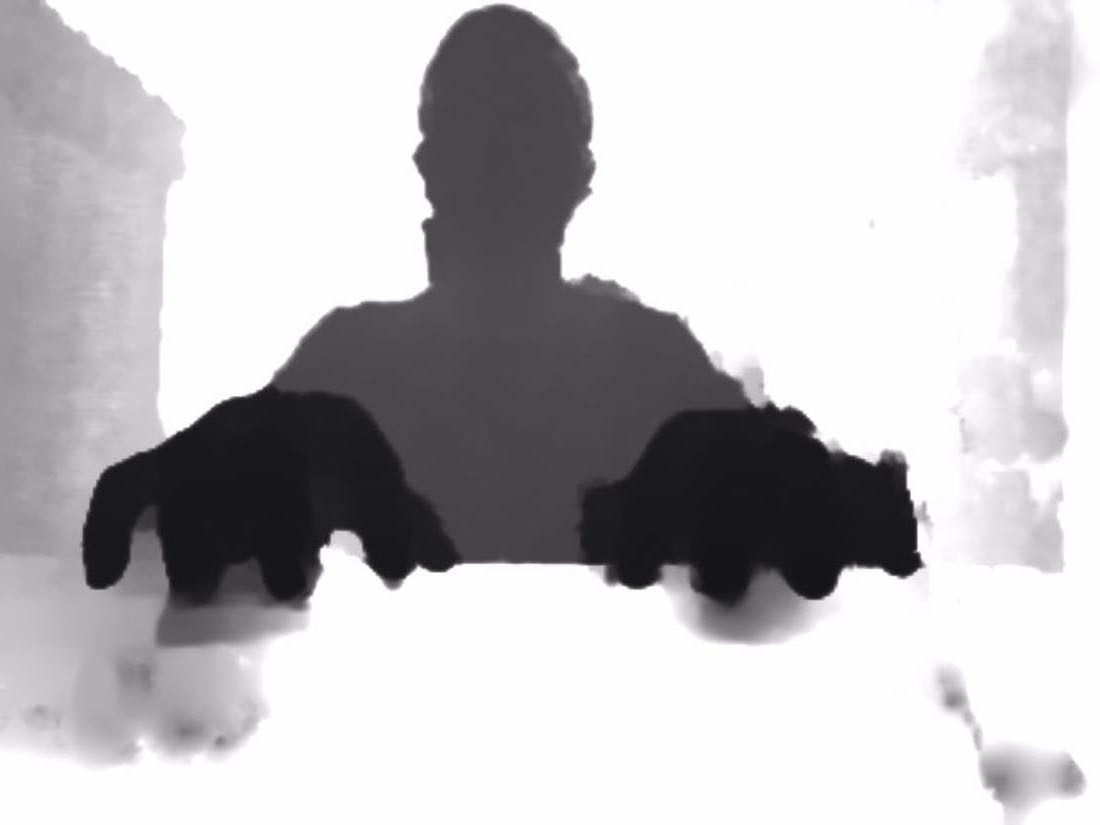
\includegraphics[height=4cm]{depth0.jpeg}}%
  \hspace{4em}%
  \subcaptionbox{处理后的深度图\label{fig:depth2}}
      {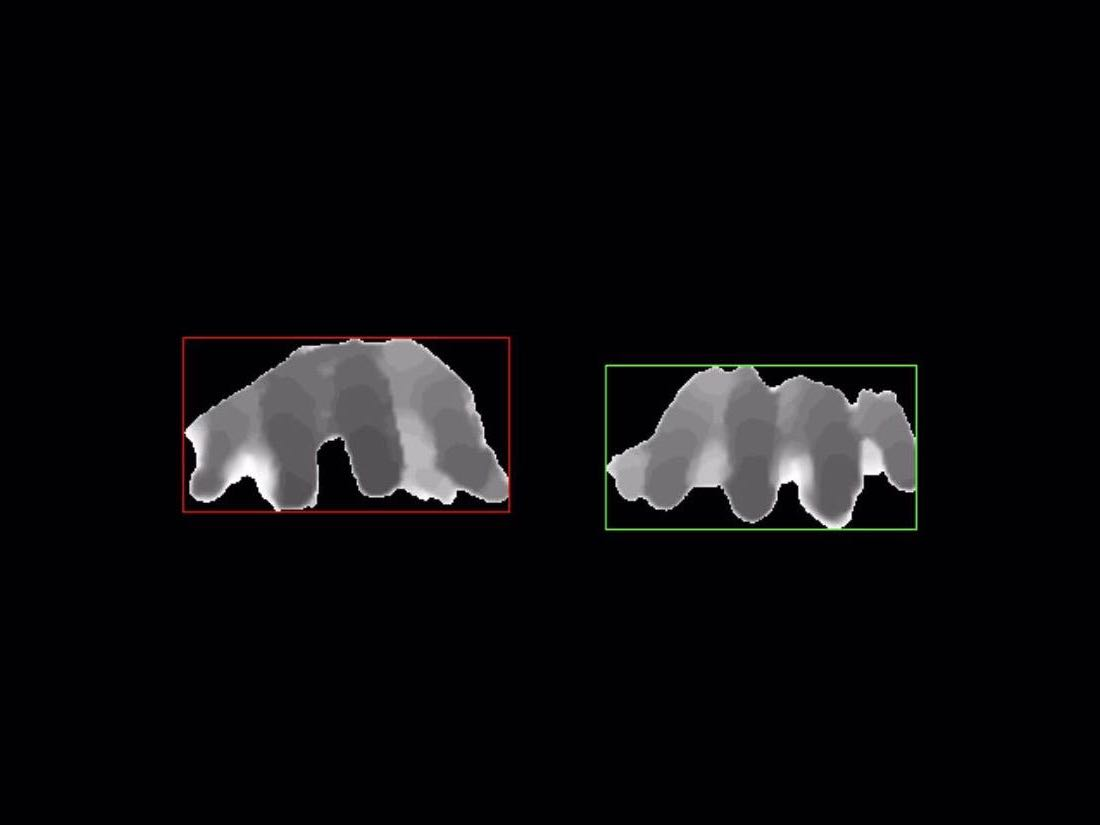
\includegraphics[height=4cm]{depth1.jpeg}}
  \caption{处理前后的深度图像}
  \label{fig:depth-image}
\end{figure}

获取处理后的深度图像后,我们首先识别出图中所有的轮廓,其中面积最大的两个即为用户的手部。当用户手部从悬浮状态发生点击时,点击的手指会位于深度图像最低点。基于这一事实,当通过声音检测到点击时,我们首先寻找到手部轮廓和外接矩形的最低点。

在图中找到最低点后,接下来便是计算点击位置离手机的距离。根据我们的尝试,由于指缝等的干扰,直接在深度图中读取点击处的像素深度可能会出现一定的误差,因此我们在该位置的领域进行洪范后计算距离的平均值。如果出现识别出多个切点的情况,我们选择距离最近的一个。

此外,基于深度图像的信息,我们不仅可以区分双手,同时还能够监测手部的运动状态,提供了左手左移和右手右移的手势。
%ring queue
%手指识别

\section{三维坐标的计算}
前面部分已经提到了如何计算点击和手机的距离,本节将介绍如何进一步计算该点击在物理世界中的三维坐标。

相机的成像,简言之,指的是将现实世界三维空间中的点映射成为图片中二维空间中的点这一过程,即将世界坐标系中的三维坐标转化为像素坐标系的二维坐标。其原理可以用式~(\ref{imageform})表示。
% 为了获得该过程的映射关系,一般需要引入以下几个坐标系:
% \begin{itemize}
%     \item \textbf{世界坐标系:}指的是物体在三维世界中的位置,一般由相机指定,用$(U, V, W)$表示
%     \item \textbf{相机坐标系:}以相机的光心为坐标系原点,到成像平面的距离为焦距,可由世界坐标系旋转和平移得到,用$(X, Y, Z)$表示
%     \item \textbf{图像坐标系:}在成像平面上的二维坐标系,用$(x, y)$表示
%     \item \textbf{像素坐标系:}最终图片的像素坐标,也在成像平面上,由图像坐标系平移和缩放得到,用$(u, v)$表示
% \end{itemize}

\begin{equation}
    \label{imageform}
    \begin{aligned}
    \begin{bmatrix}
        u \\
        v \\
        1
    \end{bmatrix}
    &= \frac{1}{Z} \begin{bmatrix}
        f / s_x & 0 & o_x & 0\\
        0 & f / s_y & o_y & 0 \\
        0 & 0 & 1 & 0
      \end{bmatrix}
      \begin{bmatrix}
        R & t \\
        0^{T} & 1
      \end{bmatrix}
      \begin{bmatrix}
        U \\
        V \\
        W \\
        1
      \end{bmatrix} \\
    &= \frac{1}{Z} \begin{bmatrix}
        f / s_x & 0 & o_x & 0\\
        0 & f / s_y & o_y & 0 \\
        0 & 0 & 1 & 0
      \end{bmatrix}
      \begin{bmatrix}
        X \\
        Y \\
        Z \\
        1
      \end{bmatrix}
    \end{aligned}
\end{equation}

式~(\ref{imageform})中的$(X, Y, Z)$为我们要求的点击在物理世界中的坐标,而$(u, v)$则是我们前文获得的点击在深度图像中的位置。$f$,$s_x$,$s_y$,$o_x$,$o_y$,$R$,$t$都属于相机的参数,可通过对应接口获取。

在本工作中,我们已经得到了点击位置在世界坐标系中的深度坐标$Z$。此外,在我们的设备中,相机坐标系和世界坐标系只是将$X, Y$调换为$V, U$。因此,前述的公式可以化简为公式~(\ref{equ:world-coord})。这样,我们便得到了一次点击的全部三维信息。由于我们在使用时手机靠于墙壁,和桌面垂直,即$Y$方向垂直桌面,因此$Y$坐标基本为定值。后文中主要用到$X$和$Z$方向坐标,为了表述方便,仍然称之为横轴和纵轴。
\begin{equation}
  \begin{aligned}
  X &= \frac{(u - o_x)s_x}{f_x} \times Z \\
  Y &= \frac{(v - o_y)s_y}{f_y} \times Z
  \end{aligned}
  \label{equ:world-coord}
\end{equation}

\section{点击识别算法流程}
根据本章前面部分描述的声音信号和深度图像处理的内容,我们可以搭建出整个的点击识别算法框架,表述为伪代码如下。

算法首先通过声音识别点击,然后查看双手是否在合适的范围内,如果有手势则先处理手势,没有手势则计算点击坐标。
\begin{algorithm}[h]
  \caption{点击识别算法伪代码} %算法的名字
  \hspace*{0.02in} {\bf Input:} %算法的输入, \hspace*{0.02in}用来控制位置,同时利用 \\ 进行换行
  声音数据流、深度数据流\\
  \hspace*{0.02in} {\bf Output:} %算法的结果输出
  点击的世界坐标
  \begin{algorithmic}[1]
  % \State some description % \State 后写一般语句
  \If{Tap Detected}
    \If{Hands in Range}
      \If{Gestures Detected}
        \State Process gestures
      \Else
        \State Find the tangent point of hand contour and its bounding box
        \State Calculate the tap coordinate in world coordinate system
        \State \Return tap coordinate
      \EndIf
    \Else 
      \State Marked as invalid tap 
      \State \Return
    \EndIf
  \EndIf
  % \For{condition} % For 语句,需要和EndFor对应
  %   \State ...
  %   \If{condition} % If 语句,需要和EndIf对应
  %     \State ...
  %   \Else
  %     \State ...
  %   \EndIf
  % \EndFor
  % \While{condition} % While语句,需要和EndWhile对应
  %   \State ...
  % \EndWhile
  % \State \Return result
  \end{algorithmic}
\end{algorithm}